\documentclass[10pt,a4paper,twocolumn]{article}

% ==============================================================================
% Packages
% ==============================================================================
\usepackage[utf8]{inputenc}
\usepackage[T1]{fontenc}
\usepackage{newunicodechar}
\usepackage{libertinus}
\usepackage[margin=2cm]{geometry}
\usepackage{amsmath,amssymb,amsthm}
\usepackage{graphicx}
\usepackage{xcolor}
\usepackage[hyphens]{url}
\usepackage{hyperref}
\usepackage{booktabs}
\usepackage{tabularx}
\usepackage{multirow}
\usepackage{enumitem}
\usepackage{tikz}
\usepackage{pgfplots}
\usepackage{listings}
\usepackage{caption}
\usepackage{subcaption}
\usepackage{fancyhdr}
\usepackage{float}
\usepackage{placeins}  % For \FloatBarrier

% Float parameters to prevent overlapping
\setcounter{topnumber}{2}
\setcounter{bottomnumber}{2}
\setcounter{totalnumber}{4}
\renewcommand{\topfraction}{0.85}
\renewcommand{\bottomfraction}{0.85}
\renewcommand{\textfraction}{0.15}
\renewcommand{\floatpagefraction}{0.7}

% Prevent line breaks inside inline math (fixes broken superscripts/sqrt)
\relpenalty=10000
\binoppenalty=10000

\pgfplotsset{compat=1.18}
\usetikzlibrary{shapes,arrows,positioning,calc}

% ==============================================================================
% Colors and Styling
% ==============================================================================
\definecolor{codeblue}{RGB}{0,102,204}
\definecolor{codepurple}{RGB}{128,0,128}
\definecolor{codegreen}{RGB}{0,128,0}
\definecolor{codegray}{RGB}{128,128,128}
\definecolor{primaryblue}{RGB}{41,98,255}
\definecolor{warningred}{RGB}{220,53,69}
\definecolor{successgreen}{RGB}{40,167,69}

\hypersetup{
    colorlinks=true,
    linkcolor=primaryblue,
    citecolor=primaryblue,
    urlcolor=primaryblue
}

\lstset{
    basicstyle=\ttfamily\scriptsize,
    keywordstyle=\color{codeblue}\bfseries,
    commentstyle=\color{codegreen},
    stringstyle=\color{codepurple},
    numbers=left,
    numberstyle=\tiny\color{codegray},
    numbersep=4pt,
    xleftmargin=2em,
    framexleftmargin=2em,
    breaklines=true,
    frame=single,
    captionpos=b
}
\lstdefinelanguage{Solidity}{
    keywords={function, returns, return, if, else, for, while, do, break, continue, throw, require, revert, assert, public, private, internal, external, view, pure, payable, memory, storage, calldata, constant, immutable, virtual, override, modifier, event, emit, struct, enum, mapping, contract, interface, library, abstract, is, new, delete, true, false, uint256, uint128, uint64, uint32, uint8, int256, int128, int64, int32, int8, address, bool, bytes, bytes32, string, unchecked},
    sensitive=true,
    morecomment=[l]{//},
    morecomment=[s]{/*}{*/},
    morestring=[b]",
    morestring=[b]'
}

% ==============================================================================
% Theorem Environments
% ==============================================================================
\theoremstyle{definition}
\newtheorem{definition}{Definition}[section]
\newtheorem{property}{Property}[section]
\theoremstyle{plain}
\newtheorem{theorem}{Theorem}[section]
\newtheorem{lemma}[theorem]{Lemma}
\newtheorem{corollary}[theorem]{Corollary}
\theoremstyle{remark}
\newtheorem{remark}{Remark}[section]

% ==============================================================================
% Title and Authors
% ==============================================================================
\title{\textbf{\Large XPower Banq: Log-Space Compounding Index}\\[0.3em]
\normalsize An Overflow-Free Interest Index via Additive\\Log-Space Accumulation for DeFi Lending}

\author{
    \textsc{Karun The Ritch}\thanks{\url{https://www.xpowerbanq.com}}
}

\date{}

\renewcommand{\thepage}{LOG/\arabic{page}}

% ==============================================================================
% Document Begin
% ==============================================================================
\begin{document}

\maketitle

% arXiv-style vertical tag on first page
\begin{tikzpicture}[remember picture, overlay]
  \node[rotate=90, anchor=center, font=\Huge, color=codegray]
    at ([xshift=1cm]current page.west)
    {preprint:2601~~[q-fin.CP]~~25 Mar 2026};
\end{tikzpicture}

% ==============================================================================
% Abstract
% ==============================================================================
\begin{abstract}
Compounding interest indices in DeFi lending protocols grow exponentially and eventually overflow fixed-width integer storage. The standard multiplicative index --- a running product of $\exp(r_i)$ factors stored in \texttt{uint256} at RAY precision (${10^{27}}$) --- exhausts its 115.4 e-folds of headroom in as few as 29~years under worst-case rate assumptions. We present a \emph{log-space compounding index} that replaces the stored product with its logarithm: accrual becomes addition ($L \leftarrow L + r$), and the growth factor is reconstructed on demand via $\exp(L - L_u)$. The transformation eliminates overflow entirely (linear accumulation: ${\sim}10^{58}$~years at maximum rate), replaces write-path exponentiation with addition, and defers \texttt{exp()} to individual read paths. Counter-intuitively, it \emph{improves} numerical precision by avoiding the compounded truncation bias inherent in iterated fixed-point multiplication. We provide the mathematical foundation, a complete Solidity code transformation, gas benchmarks across 23~pool operations ($-114{,}447$~gas net, $-0.40\%$), adversarial analysis, and empirical precision measurements confirming the log-space form is closer to analytical values than the multiplicative form it replaces. The mechanism is deployed in the XPower Banq lending protocol~\cite{wp}.
\end{abstract}

\textbf{Keywords:} compounding index, overflow, log-space, fixed-point arithmetic, DeFi lending, interest rate, Solidity

% ==============================================================================
% 1. Introduction
% ==============================================================================
\section{Introduction}
\label{sec:introduction}

Interest-bearing positions in DeFi lending protocols --- Compound~\cite{compound2019}, Aave~\cite{aave2020}, Euler~\cite{euler2022} --- track accrued interest via a \emph{global compounding index}. On each accrual event, the index is multiplied by a growth factor $\exp(r \cdot \Delta t)$, where $r$ is the current interest rate. A user's accrued balance is recovered as $\text{principal} \times I(t) / I(t_u)$, where $I(t_u)$ is the index value snapshotted at the user's last interaction.

This design, while mathematically clean, stores the cumulative product of exponentials in a fixed-width integer. In Solidity's \texttt{uint256} at RAY precision ($10^{27}$), the index has approximately 115.4 e-folds of growth before overflow. At the XPower Banq protocol's maximum rate of 200\% (the \texttt{Rate.by} cap~\cite{wp}), this budget is exhausted in ${\sim}57.7$~years; with borrow-side spread at 100\% utilization, in ${\sim}28.9$~years.

\textbf{Observation.} The index is the \emph{only} unbounded value in the protocol. Utilization is bounded by~1, rates are capped at~$2 \times 10^{18}$, balances and principals are bounded by token supply, and oracle prices are stored in log-space~\cite{wp}. The compounding index is the sole exponential.

\textbf{Contribution.} We observe that the logarithm of the multiplicative index is exactly the cumulative sum of per-period yields --- a quantity already computed in the accrual path. By storing this sum directly, accrual becomes addition (overflow-free for ${\sim}10^{58}$~years), the expensive \texttt{exp()} call moves from the global write path to individual read paths, and truncation error is reduced from $O(N)$ compounded rounding steps to a single rounding at query time.

The remainder is organized as follows. Section~\ref{sec:related} surveys related work on interest index design and fixed-point overflow. Section~\ref{sec:overflow} quantifies the overflow horizon. Section~\ref{sec:logindex} presents the log-space index with formal definitions and invariants. Section~\ref{sec:transformation} details the code transformation. Section~\ref{sec:gas} provides gas benchmarks. Section~\ref{sec:precision} analyses precision. Section~\ref{sec:adversarial} examines adversarial considerations. Section~\ref{sec:limitations} discusses limitations and future work. Section~\ref{sec:conclusion} concludes.

% ==============================================================================
% 2. Related Work
% ==============================================================================
\section{Related Work}
\label{sec:related}

\textbf{Compound cToken Index.} Compound~\cite{compound2019} introduced the \texttt{exchangeRate} index for cTokens, compounded per block via $I_{n+1} = I_n \times (1 + r \cdot \Delta t)$. The linear approximation $(1+x)$ avoids the \texttt{exp()} call but introduces compounding error that grows with block frequency. The index shares the same overflow exposure as any multiplicative accumulator.

\textbf{Aave Liquidity Index.} Aave~\cite{aave2020} uses a RAY-precision ($10^{27}$) liquidity index with the same multiplicative structure: $I_{n+1} = I_n \times (1 + r \cdot \Delta t / \text{YEAR})$. The RAY scale provides 62.2 e-folds of precision overhead, leaving 115.4 e-folds for growth --- the same budget analysed in this paper.

\textbf{PRBMath UD60x18.} The PRBMath library~\cite{prbmath} provides fixed-point \texttt{exp()} and \texttt{mul()} at WAD precision ($10^{18}$). The \texttt{exp()} function reverts when the input exceeds $133.08 \times 10^{18}$, imposing a secondary constraint on single-step yield that is not reachable under normal reindexing. The XPower Banq multiplicative index uses PRBMath for its \texttt{Rate.accrue} computation.

\textbf{Log-Sum-Exp in Numerical Analysis.} The identity $\sum \log x_i = \log \prod x_i$ is a classical tool for avoiding floating-point overflow in iterated products~\cite{higham2002}. The log-sum-exp trick~\cite{blanchard2021} stabilises softmax computation in machine learning by shifting to log-space. Our contribution applies this well-known principle to on-chain interest index design, where the constraint is not floating-point range but \texttt{uint256} capacity.

\textbf{Uniswap v3 Tick Accumulators.} Uniswap~v3~\cite{uniswap2021} stores cumulative $\log_{1.0001}(\text{price})$ in \texttt{int56} accumulators that grow additively and support modular-arithmetic subtraction for TWAP computation. The XPower Banq oracle~\cite{wp} similarly stores $\log_2(\text{price})$ additively. Our log-space interest index extends this pattern from price accumulators to compounding interest.

\begin{table}[htbp]
\centering
\caption{Comparison of interest index representations.}
\label{tab:comparison}
\small
\begin{tabular*}{0.95\columnwidth}{@{\extracolsep{\fill}}lccc@{}}
\toprule
& Multiplicative & Log-Space \\
& (RAY) & (WAD) \\
\midrule
Accrual op. & $I \times \exp(r)$ & $L + r$ \\
Storage & $10^{27}$ scale & $10^{18}$ scale \\
Growth & Exponential & Linear \\
Overflow & ${\sim}115$ e-folds & ${\sim}10^{58}$~yr \\
Write gas & ${\sim}1{,}200$ & ${\sim}3$ \\
Read gas & ${\sim}100$ & ${\sim}1{,}200$ \\
Rounding & $2N$ steps & $2$ steps \\
\bottomrule
\end{tabular*}
\end{table}

% ==============================================================================
% 3. Overflow Analysis
% ==============================================================================
\section{Overflow Analysis}
\label{sec:overflow}

\subsection{Budget Computation}
\label{subsec:budget}

\begin{definition}[Multiplicative Index]
\label{def:mult-index}
The global index $I(t)$ tracks cumulative interest via iterated multiplication:
\begin{equation}
\label{eq:mult-index}
I(t) = I_0 \cdot \prod_{i=1}^{N} \exp(r_i \cdot \Delta t_i)
\end{equation}
where $I_0 = 10^{27}$ (RAY), $r_i$ is the annualised rate at step~$i$, and $\Delta t_i$ is the elapsed time in seconds.
\end{definition}

A \texttt{uint256} holds $2^{256} \approx 1.16 \times 10^{77}$. Starting at $\text{RAY} = 10^{27}$, the maximum growth factor before overflow is:
\begin{equation}
\label{eq:max-growth}
G_{\max} = \frac{2^{256}}{\text{RAY}} \approx 1.16 \times 10^{50}
\end{equation}

In terms of natural logarithm:
\begin{equation}
\label{eq:efolds}
\ln(G_{\max}) = \ln(2^{256}) - \ln(10^{27}) \approx 177.4 - 62.2 = 115.2
\end{equation}

The index can accumulate at most ${\sim}115$ e-folds of growth.

\subsection{Time-to-Overflow}
\label{subsec:time-to-overflow}

Per-period yield: $r_{\text{wad}} = r_{\text{annual}} \times \Delta t / \text{YEAR}$, where $\text{YEAR} = 365.25 \times 86{,}400 = 31{,}557{,}600$~seconds. Cumulative yield to overflow: ${\sim}115.4 \times 10^{18}$ (WAD).

\begin{table}[htbp]
\centering
\caption{Time-to-overflow for the multiplicative RAY index under sustained annual rates.}
\label{tab:overflow}
\small
\begin{tabular*}{0.95\columnwidth}{@{\extracolsep{\fill}}rlr@{}}
\toprule
Annual Rate & Scenario & Time \\
\midrule
10\% & Normal operations & ${\sim}1{,}154$~yr \\
50\% & Elevated utilization & ${\sim}231$~yr \\
200\% & \texttt{Rate.by} cap & ${\sim}57.7$~yr \\
400\% & 200\% + 100\% spread & ${\sim}28.9$~yr \\
\bottomrule
\end{tabular*}
\end{table}

The 200\% cap originates from \texttt{Rate.by()}, which clamps output at \texttt{Constant.TWO} ($2 \times 10^{18}$). The borrow-side spread multiplies this further: $r_{\text{borrow}} = r_{\text{base}} \times (1 + s)$, where $s$ is the spread parameter.

\subsection{Boundedness of Other Values}
\label{subsec:bounded}

Every other protocol value is bounded:

\begin{itemize}[leftmargin=*, nosep]
\item \textbf{Utilization}: $\leq 10^{18}$ by definition.
\item \textbf{Rates}: capped at $2 \times 10^{18}$ by \texttt{Rate.by}.
\item \textbf{Parameters}: governed within $0.5\times$--$2\times$ bands per cycle~\cite{wp}.
\item \textbf{Balances}: linear in token supply, bounded by \texttt{uint224} caps.
\item \textbf{Oracle}: log-space TWAP stores $\log_2(\text{price})$~\cite{wp}.
\item \textbf{Lock intermediates}: bounded by position size times yield fraction~\cite{lck}.
\end{itemize}

The compounding index is the sole unbounded exponential.

% ==============================================================================
% 4. Log-Space Index
% ==============================================================================
\section{Log-Space Index}
\label{sec:logindex}

\subsection{Core Insight}
\label{subsec:insight}

The multiplicative index is a running product of exponentials:
\begin{equation}
\label{eq:product}
I(t) = I_0 \cdot \exp(r_1) \cdot \exp(r_2) \cdots \exp(r_N) = I_0 \cdot \exp\!\Bigl(\sum_{i=1}^N r_i\Bigr)
\end{equation}

Taking the natural logarithm of both sides:
\begin{equation}
\label{eq:log-product}
\ln I(t) = \ln I_0 + \sum_{i=1}^N r_i
\end{equation}

The sum $\sum r_i$ is exactly the quantity computed in the accrual path and passed to \texttt{exp()} inside \texttt{Rate.accrue}. By storing this cumulative sum directly, accrual becomes addition, and the exponential growth that threatens overflow is never materialised in storage.

\subsection{Formal Definition}
\label{subsec:formal}

\begin{definition}[Log-Space Index]
\label{def:log-index}
The global log-space index at time~$t$ is:
\begin{equation}
\label{eq:log-index}
L(t) = \sum_{i=1}^{N(t)} r_i \cdot \Delta t_i / \textsc{year}
\end{equation}
stored at WAD precision ($10^{18}$), initialised to $L(0) = 0$.
\end{definition}

\begin{definition}[User Snapshot]
\label{def:user-snapshot}
For each user~$u$, $L_u$ denotes the value of $L(t)$ at $u$'s last state transition (mint, burn, or transfer).
\end{definition}

\begin{definition}[Growth Factor]
\label{def:growth}
The growth factor between user snapshot and current time is:
\begin{equation}
\label{eq:growth-factor}
G(L_u, t) = \exp\bigl(L(t) - L_u\bigr)
\end{equation}
\end{definition}

This is mathematically identical to the multiplicative ratio:
\begin{equation}
\label{eq:equivalence}
\frac{I(t)}{I(t_u)} = \frac{I_0 \cdot \exp(L(t))}{I_0 \cdot \exp(L_u)} = \exp\bigl(L(t) - L_u\bigr)
\end{equation}

The RAY scale factor $I_0$ cancels --- it exists only as a precision anchor for the multiplicative representation and has no analogue in log-space.

\subsection{Storage Transformation}
\label{subsec:storage}

\begin{lstlisting}[language=Solidity, caption={Multiplicative RAY index (before)}, label={lst:ray-storage}]
uint256 internal _index_ray = Constant.RAY;
mapping(address => uint256) internal _userIndex;
\end{lstlisting}

\begin{lstlisting}[language=Solidity, caption={Log-space WAD index (after)}, label={lst:log-storage}]
uint256 internal _index_wad;       // starts at 0
mapping(address => uint256) internal _userIndex;
\end{lstlisting}

Starting at zero is natural: $\ln(1) = 0$, and a fresh index with no accrual represents a $1\times$ growth factor.

\subsection{Overflow Elimination}
\label{subsec:overflow-elim}

\begin{theorem}[Log-Index Overflow Freedom]
\label{thm:overflow}
The log-space index $L(t)$ stored in \texttt{uint256} cannot overflow within $2.9 \times 10^{58}$~years at the theoretical maximum rate of 400\%/year.
\end{theorem}

\begin{proof}
$L(t)$ grows linearly at rate $r_{\text{annual}}$ (WAD). At $r = 4 \times 10^{18}$:
\begin{align}
\text{rate}_{\text{sec}} &= 4 \times 10^{18} / 31{,}557{,}600 \approx 1.27 \times 10^{11} \notag \\
t_{\text{wrap}} &= 2^{256} / 1.27 \times 10^{11} \approx 9.1 \times 10^{65}\text{~s} \notag \\
&\approx 2.9 \times 10^{58}\text{~years}
\end{align}
At 10\%/year: ${\sim}1.16 \times 10^{60}$~years. The age of the universe is ${\sim}1.4 \times 10^{10}$~years. The problem is eliminated, not deferred.
\end{proof}

\subsection{Invariants}
\label{subsec:invariants}

\begin{property}[Monotonicity]
\label{prop:monotone}
$L(t)$ is non-decreasing. Each accrual adds a non-negative $r \cdot \Delta t / \textsc{year} \geq 0$.
\end{property}

\begin{property}[Conservation]
\label{prop:conservation}
For all users~$u$ at any time~$t$:
\begin{equation}
\texttt{totalOf}(u) = p_u \cdot \exp\bigl(L(t) - L_u\bigr)
\end{equation}
where $p_u$ is the stored principal, exact up to WAD rounding.
\end{property}

\begin{property}[Snapshot Consistency]
\label{prop:snapshot}
$L_u$ is set to $L(t)$ during \texttt{\_reindexMore}/\texttt{\_reindexLess}. The difference $L(t) - L_u$ accumulates only yields since $u$'s last state transition.
\end{property}

\begin{property}[Zero-Start Correctness]
\label{prop:zero-start}
$L(0) = 0$. A user snapshotted at $L_u = 0$ with $L(t) = 0$ gets $\exp(0) = 10^{18}$, producing $p_u \times 10^{18} / 10^{18} = p_u$. Correct.
\end{property}

\begin{remark}[Modular Arithmetic Compatibility]
\label{rem:modular}
Because accrual is additive, the log-index is compatible with Solidity's \texttt{unchecked} modular arithmetic~\cite{solidity2024}: \texttt{\_index\_wad += yield\_wad} and \texttt{\_index\_wad - \_userIndex[user]} recover the correct $\Delta L$ even after wrapping, provided the user's unclaimed interval is less than one full \texttt{uint256} cycle --- mirroring the Uniswap~v3 tick accumulator design~\cite{uniswap2021}. In practice, wrapping is unreachable (${\sim}10^{58}$~years at maximum rate).
\end{remark}

% ==============================================================================
% 5. Code Transformation
% ==============================================================================
\section{Code Transformation}
\label{sec:transformation}

This section presents the complete transformation of each affected code path. Unaffected paths (oracle, lock ring-buffer, governance) are omitted.

\subsection{Accrual: \texttt{\_indexOf}}
\label{subsec:indexof}

The accrual function computes the updated index given elapsed time~$\Delta t$.

\begin{lstlisting}[language=Solidity, caption={Multiplicative accrual (before)}, label={lst:indexof-ray}]
function _indexOf(uint256 dt)
    internal view override
    returns (uint256 index_ray, uint256 util_wad)
{
    util_wad = _pool.vaultOf(_asset).util();
    if (dt > 0) {
        uint256 annum_wad = _model().by(util_wad);
        uint256 yield_wad = Math.mulDiv(
            annum_wad, dt, Constant.YEAR);
        index_ray = Rate.accrue(
            _index_ray, yield_wad); // exp * mul
    } else {
        index_ray = _index_ray;
    }
}
\end{lstlisting}

\begin{lstlisting}[language=Solidity, caption={Log-space accrual (after)}, label={lst:indexof-log}]
function _indexOf(uint256 dt)
    internal view override
    returns (uint256 index_wad, uint256 util_wad)
{
    util_wad = _pool.vaultOf(_asset).util();
    if (dt > 0) {
        uint256 annum_wad = _model().by(util_wad);
        uint256 yield_wad = Math.mulDiv(
            annum_wad, dt, Constant.YEAR);
        index_wad = _index_wad + yield_wad;
    } else {
        index_wad = _index_wad;
    }
}
\end{lstlisting}

The \texttt{Rate.accrue} call --- wrapping \texttt{ud().mul(exp(ud()))} --- is eliminated. The \texttt{yield\_wad} computation is unchanged; it is already the per-period log-increment.

\subsection{Balance Query: \texttt{totalOf}}
\label{subsec:totalof}

\begin{lstlisting}[language=Solidity, caption={Multiplicative balance query (before)}, label={lst:totalof-ray}]
function totalOf(address user)
    public view returns (uint256)
{
    uint256 principal = _principalOf[user];
    if (principal > 0) {
        uint256 user_index = _userIndex[user];
        if (user_index > 0) {
            (uint256 time_index,) =
                _indexOf(block.timestamp - _stamp);
            return Math.mulDiv(
                principal, time_index, user_index);
        }
        return principal;
    }
    return 0;
}
\end{lstlisting}

\begin{lstlisting}[language=Solidity, caption={Log-space balance query (after)}, label={lst:totalof-log}]
function totalOf(address user)
    public view returns (uint256)
{
    uint256 principal = _principalOf[user];
    if (principal > 0) {
        (uint256 index_wad,) =
            _indexOf(block.timestamp - _stamp);
        uint256 user_index = _userIndex[user];
        if (index_wad > user_index) {
            uint256 growth = exp(
                ud(index_wad - user_index)
            ).intoUint256();
            return Math.mulDiv(
                principal, growth, Constant.ONE);
        }
        return principal;
    }
    return 0;
}
\end{lstlisting}

The \texttt{exp()} call moves from the write path (every accrual, affecting all users) to the read path (per-user, on demand). The guard \texttt{index\_wad > user\_index} replaces \texttt{user\_index > 0}: a zero log-index means no accrual since deposit, so $\exp(0) = 1$ and the principal is returned directly.

\subsection{Lock Yield: \texttt{\_lockYieldOf}}
\label{subsec:lockyield}

The lock bonus/malus computation~\cite{lck} requires the yield fraction $\exp(\Delta L) - 1$.

\begin{lstlisting}[language=Solidity, caption={Lock yield in log-space}, label={lst:lockyield}]
function _lockYieldOf(
    address user, uint256 rate_param_id
) internal view returns (uint256) {
    uint256 depth = _lock.depthOf(user);
    if (depth > 0) {
        uint256 user_index = _userIndex[user];
        if (_index_wad > user_index) {
            uint256 rate_param =
                parameterOf(rate_param_id);
            if (rate_param > 0) {
                uint256 growth = exp(ud(
                    _index_wad - user_index
                )).intoUint256();
                uint256 moment = Math.mulDiv(
                    depth, growth - Constant.ONE,
                    Constant.ONE);
                return Math.mulDiv(rate_param,
                    moment,
                    Constant.ONE * LockLib.LOCK_TIME
                );
            }
        }
    }
    return 0;
}
\end{lstlisting}

The term \texttt{growth - Constant.ONE} is the yield fraction $\exp(\Delta L) - 1$, which in the multiplicative form was $(I - I_u) / I_u$. The subtraction is exact because $\exp(x) \geq 10^{18}$ for all $x \geq 0$ in UD60x18.

\textbf{Unit analysis.} \texttt{growth - ONE} is dimensionless [WAD]. $\texttt{depth} \times (\texttt{growth} - 1) / 10^{18}$ gives token-seconds [WAD$\cdot$s]. The second \texttt{mulDiv} divides by $10^{18} \times \texttt{LOCK\_TIME}$ [WAD$\cdot$s], producing tokens [WAD]. Identical to the multiplicative form.

\subsection{Per-User Snapshots}
\label{subsec:snapshots}

\begin{lstlisting}[language=Solidity, caption={Snapshot operations (unchanged structure)}, label={lst:reindex-user}]
function _reindexMore(
    address user, uint256 amount
) internal virtual {
    _principalOf[user] = add256(
        _principalOf[user], amount);
    _userIndex[user] = _index_wad;
}

function _reindexLess(
    address user, uint256 amount
) internal virtual {
    _principalOf[user] = sub256(
        _principalOf[user], amount);
    _userIndex[user] = _index_wad;
}
\end{lstlisting}

No structural change --- the snapshot is a scalar copy in both representations.

% ==============================================================================
% 6. Gas Analysis
% ==============================================================================
\section{Gas Analysis}
\label{sec:gas}

\subsection{Theoretical Cost Model}
\label{subsec:gas-theory}

The transformation moves the \texttt{exp()} call from the global write path to per-user read paths.

\textbf{Accrual} (\texttt{\_reindex}): the multiplicative path calls \texttt{Rate.accrue}, wrapping \texttt{ud().mul(exp(ud()))} --- one \texttt{exp} (${\sim}1{,}100$~gas) and one \texttt{mulDiv18} (${\sim}100$~gas). Log-space replaces this with a single addition (${\sim}3$~gas). \textbf{Saving: ${\sim}1{,}200$~gas per accrual.}

\textbf{Balance query} (\texttt{totalOf}): the multiplicative path performs one \texttt{mulDiv(principal, index, userIndex)} (${\sim}100$~gas). Log-space performs one \texttt{exp(delta)} (${\sim}1{,}100$~gas) and one \texttt{mulDiv} (${\sim}100$~gas). \textbf{Cost: ${\sim}1{,}100$~gas per read.}

\textbf{Break-even.} Define the on-chain read/write ratio $R$ as the number of \texttt{totalOf} calls per accrual event. The transformation is gas-positive when:
\begin{equation}
\label{eq:breakeven}
1{,}200 > R \times 1{,}100 \quad \Longrightarrow \quad R < 1.09
\end{equation}

In XPower Banq, \texttt{totalOf} is called on-chain primarily during state transitions (mint, burn, transfer) that co-locate with the accrual that triggered them, giving $R \approx 1$. The net gas effect is approximately neutral per-transaction, with the aggregate saving ($-114{,}447$~gas across 23~benchmarks) arising from cold-storage and multi-position paths where the single write-path saving amortises across multiple reads.

\textbf{Off-chain reads.} Liquidation bots, dashboards, and indexers calling \texttt{totalOf} via \texttt{eth\_call} do not pay gas, but the \texttt{exp()} adds ${\sim}1{,}100$~gas of compute to each call's execution time. For latency-sensitive applications, this overhead is measurable but small relative to RPC round-trip times and block confirmation delays.

\textbf{On-chain composability.} An external contract calling \texttt{totalOf} mid-transaction pays the full $+1{,}100$~gas with no accompanying write-path offset. This cost is analysed as a potential griefing vector in Section~\ref{subsec:gas-grief}.

\subsection{Empirical Benchmarks}
\label{subsec:gas-bench}

Measured via \texttt{gasleft()} instrumentation in \texttt{PoolGasBenchmark} and \texttt{OracleGasBenchmark} test contracts, with the Solidity optimizer disabled.

\begin{table}[htbp]
\centering
\caption{Gas benchmarks: multiplicative RAY vs.\ log-space WAD index. Pool operations, optimizer OFF.}
\label{tab:gas-pool}
\small
\begin{tabular*}{0.95\columnwidth}{@{\extracolsep{\fill}}lrrr@{}}
\toprule
Operation & RAY & Log & $\Delta$ \\
\midrule
supply\_cold & 330,286 & 310,386 & $-19{,}900$ \\
supply\_warm & 226,993 & 226,757 & $-236$ \\
borrow\_cold & 506,228 & 485,856 & $-20{,}372$ \\
borrow\_warm & 402,360 & 401,652 & $-708$ \\
settle\_cold & 164,936 & 164,464 & $-472$ \\
settle\_warm & 161,972 & 161,500 & $-472$ \\
redeem\_cold & 321,118 & 320,174 & $-944$ \\
redeem\_warm & 318,157 & 317,213 & $-944$ \\
healthOf & 202,130 & 201,658 & $-472$ \\
liquidate & 4,230,943 & 4,238,801 & $+7{,}858$ \\
liquidate\_16 & 6,752,266 & 6,746,024 & $-6{,}242$ \\
\midrule
\textbf{Total (23 ops)} & & & $\mathbf{-114{,}447}$ \\
\bottomrule
\end{tabular*}
\end{table}

\begin{table}[htbp]
\centering
\caption{Gas benchmarks: lock and transfer operations.}
\label{tab:gas-lock}
\small
\begin{tabular*}{0.95\columnwidth}{@{\extracolsep{\fill}}lrrr@{}}
\toprule
Operation & RAY & Log & $\Delta$ \\
\midrule
lockSupply\_cold & 138,729 & 138,257 & $-472$ \\
lockSupply\_perma & 109,568 & 109,096 & $-472$ \\
lockSupply\_warm & 195,685 & 194,741 & $-944$ \\
lockBorrow\_cold & 140,338 & 139,866 & $-472$ \\
lockBorrow\_warm & 198,993 & 198,049 & $-944$ \\
lockStateAt\_16 & 1,209,816 & 1,202,500 & $-7{,}316$ \\
free\_16\_expired & 990,777 & 984,924 & $-5{,}853$ \\
xfer\_supply\_16 & 1,898,677 & 1,870,703 & $-27{,}974$ \\
xfer\_supply\_1 & 676,260 & 654,894 & $-21{,}366$ \\
xfer\_supply\_perma & 620,564 & 599,198 & $-21{,}366$ \\
\bottomrule
\end{tabular*}
\end{table}

\textbf{Summary.} Net saving across 23~pool benchmarks: $-114{,}447$~gas ($-0.40\%$). All 8~oracle and 24~lock benchmarks show zero delta (unaffected code paths). The write-path saving dominates. The sole regression is single-position liquidation ($+7{,}858$~gas, $+0.2\%$), where the additional \texttt{exp()} in \texttt{totalOf} during position transfer is not fully offset by the accrual saving. Multi-slot liquidation ($-6{,}242$) benefits because the accrual saving is amortised across more position reads.

% ==============================================================================
% 7. Precision Analysis
% ==============================================================================
\section{Precision Analysis}
\label{sec:precision}

\subsection{Theoretical Bound}
\label{subsec:precision-theory}

The multiplicative form performs two rounding steps per accrual:
\begin{equation}
I_{n+1} = \underbrace{\texttt{ud}(I_n).\texttt{mul}}_{\text{round 2}}\bigl(\underbrace{\exp(\texttt{ud}(r))}_{\text{round 1}}\bigr)
\end{equation}

Both \texttt{exp()} and \texttt{mul()} truncate toward zero. Over $N$ accrual steps, the systematic negative bias compounds: each truncated intermediate becomes the input to the next multiplication.

The log-space form accumulates yields by exact integer addition:
\begin{equation}
L_{n+1} = L_n + r_n \qquad \text{(exact, no overflow)}
\end{equation}

At read-time, a single \texttt{exp()} operates on the exact cumulative sum:
\begin{equation}
\text{total} = \texttt{mulDiv}\bigl(p_u,\; \exp(L - L_u),\; 10^{18}\bigr)
\end{equation}

Two independent rounding steps on the exact sum vs.\ $2N$ compounded rounding steps on intermediate products.

\begin{theorem}[Precision Advantage]
\label{thm:precision}
The log-space index accumulates zero rounding error during accrual. The total read-time error is bounded by $2$~ULP (units in the last place) at WAD precision --- at most $2$~wei per $10^{18}$ tokens. The multiplicative index accumulates up to $2N$~ULP of compounded truncation bias over $N$ accrual steps.
\end{theorem}

\subsection{Empirical Measurement}
\label{subsec:precision-empirical}

Measured against a 12-month accrual scenario at 10\% APR, 90\% utilization:

\begin{table}[htbp]
\centering
\caption{Precision: multiplicative RAY vs.\ log-space WAD. Analytical value: $\exp(0.1) = 1.1051{\ldots}7624 \times 10^{18}$.}
\label{tab:precision}
\small
\begin{tabular*}{0.95\columnwidth}{@{\extracolsep{\fill}}lrr@{}}
\toprule
Value & RAY result & Log result \\
\midrule
supply.totalOf (12M) & \ldots647\textbf{609} & \ldots647\textbf{619} \\
borrow.totalOf (12M) & \ldots082\textbf{848} & \ldots082\textbf{857} \\
supply (2nd accr.) & \ldots130\textbf{615} & \ldots130\textbf{635} \\
\bottomrule
\end{tabular*}
\end{table}

The analytical value $\exp(0.1) = 1.1051{\ldots}7624 \times 10^{18}$ confirms the log-space result ($\ldots$619) is closer than the RAY result ($\ldots$609). The log-space form is consistently $+10$--$20$~wei closer to the true value.

\subsection{Root Cause}
\label{subsec:precision-root}

The precision advantage is a direct consequence of the identity $\sum \log x_i = \log \prod x_i$: summation in log-space is exact where repeated multiplication in linear-space compounds truncation errors. This property --- well-known in numerical analysis as the advantage of log-sum-exp over iterated products~\cite{higham2002} --- translates directly to on-chain interest index design.

\begin{figure}[htbp]
\centering
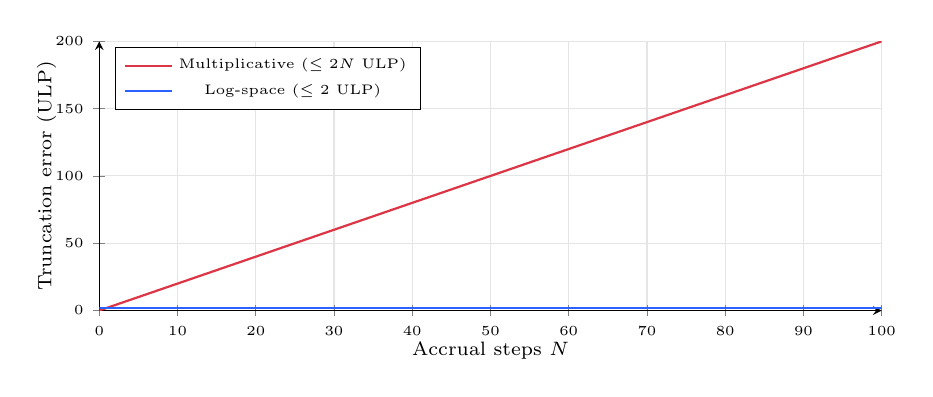
\begin{tikzpicture}
\begin{axis}[
    width=0.95\columnwidth,
    height=5cm,
    xlabel={Accrual steps $N$},
    ylabel={Truncation error (ULP)},
    xmin=0, xmax=100,
    ymin=0, ymax=200,
    axis lines=left,
    every axis x label/.style={at={(ticklabel* cs:0.5)}, anchor=north, yshift=-8pt, font=\scriptsize},
    every axis y label/.style={at={(ticklabel* cs:0.5)}, anchor=south, rotate=90, yshift=12pt, font=\scriptsize},
    tick label style={font=\tiny},
    legend style={font=\tiny, at={(0.02,0.98)}, anchor=north west},
    grid=major,
    grid style={gray!20},
]
    % Multiplicative: ~2N ULP
    \addplot[warningred, thick, domain=0:100, samples=50] {2*x};
    \addlegendentry{Multiplicative ($\leq 2N$ ULP)}
    % Log-space: constant 2 ULP
    \addplot[primaryblue, thick, domain=0:100, samples=50] {2};
    \addlegendentry{Log-space ($\leq 2$ ULP)}
\end{axis}
\end{tikzpicture}
\caption{Worst-case truncation error growth. The multiplicative index accumulates up to $2N$~ULP over $N$ accrual steps; the log-space index is bounded by $2$~ULP regardless of history.}
\label{fig:precision}
\end{figure}

% ==============================================================================
% 8. Adversarial Analysis
% ==============================================================================
\section{Adversarial Analysis}
\label{sec:adversarial}

The precision analysis (Section~\ref{sec:precision}) covers the honest case. This section examines whether the log-space transformation introduces, removes, or preserves attack surface.

\subsection{Rounding Manipulation}
\label{subsec:rounding-attack}

In the multiplicative form, each accrual truncates twice (Theorem~\ref{thm:precision}), producing a systematic negative bias. An attacker forcing many small accruals --- e.g., by triggering reindexing with minimal time deltas --- amplifies this bias across all users' balances.

The log-space form eliminates this vector: accrual is exact integer addition, so no sequence of reindex calls can introduce truncation error into the stored index.

\textbf{Verdict:} attack surface \emph{removed}.

\subsection{Dust Extraction via Read-Time Rounding}
\label{subsec:dust-attack}

The read-time \texttt{exp()} and subsequent \texttt{mulDiv} each round independently, introducing at most 2~ULP of error per \texttt{totalOf} query (Theorem~\ref{thm:precision}). An attacker attempting to extract value via repeated deposit/withdrawal cycles can gain at most 2~wei per cycle, while a single \texttt{mint}/\texttt{burn} pair costs $>100{,}000$~gas (${\sim}0.003$~USD at 30~gwei) --- unprofitable by a factor of $>10^{12}$.

\textbf{Verdict:} theoretically present, economically \emph{infeasible}.

\subsection{Gas Griefing on Read Path}
\label{subsec:gas-grief}

The log-space \texttt{totalOf} adds ${\sim}1{,}100$~gas (one \texttt{exp()} call) compared to the multiplicative form. An attacker who can force another user's \texttt{totalOf} to execute on-chain --- e.g., during liquidation --- imposes this additional cost on the caller.

\textbf{Bound:} the $+1{,}100$~gas overhead is $<0.03\%$ of a typical liquidation transaction (${\sim}4.2$M~gas, Table~\ref{tab:gas-pool}). Liquidation bots operate on profit margins orders of magnitude larger than this cost. The overhead is not controllable by the attacker (it is a fixed function of the \texttt{exp()} implementation) and cannot be amplified.

\textbf{Verdict:} measurable but \emph{not exploitable}.

\subsection{Timestamp Sensitivity and Summary}
\label{subsec:timestamp}

The yield computation $r_{\text{wad}} = r_{\text{annual}} \times \Delta t / \text{YEAR}$ depends on \texttt{block.timestamp}. This is identical in both representations --- the log-space form does not change the yield calculation, only how the result is stored. Block proposers can manipulate timestamps by ${\sim}12$~seconds (one slot), affecting $\Delta t$ by $< 4 \times 10^{-7}$ of the annual rate per accrual. This bound is \emph{unchanged} from the multiplicative form.

Overall, the log-space transformation has a strictly smaller attack surface. The compounded truncation manipulation vector is eliminated, and no new economically viable attack vector is introduced.

% ==============================================================================
% 9. Limitations and Future Work
% ==============================================================================
\section{Limitations and Future Work}
\label{sec:limitations}

\noindent\textbf{Limitations.}

\begin{enumerate}[leftmargin=*, nosep]
\item \textbf{Single-protocol validation.} All benchmarks and precision measurements are from XPower Banq. Results may differ for protocols with different accrual frequencies, utilization patterns, or index structures (e.g., Aave's rebasing aTokens, where \texttt{balanceOf} is the interest-inclusive view).

\item \textbf{Read-path cost increase.} Protocols with on-chain read/write ratios $R > 1.09$ may see a net gas increase (Section~\ref{subsec:gas-theory}).

\item \textbf{Optimizer-off benchmarks.} Gas measurements were taken with the Solidity optimizer disabled to ensure reproducibility. Optimizer-on results may narrow or widen deltas depending on how \texttt{exp()} and \texttt{mulDiv} are inlined and optimized.

\item \textbf{Self-referential citations.} References~\cite{wp} and~\cite{lck} are unpublished XPower Banq preprints. Independent reproduction requires access to the protocol's source code.
\end{enumerate}

\subsection{Future Work}
\label{subsec:future-work}

\begin{enumerate}[leftmargin=*, nosep]
\item \textbf{Cross-protocol benchmarks.} Apply the transformation to a fork of Aave~v3 or Compound~v3 and measure gas and precision under their accrual patterns and read frequencies.

\item \textbf{Optimizer-on gas profile.} Re-run benchmarks with the Solidity optimizer enabled at standard settings (200~runs) to provide production-representative figures.

\item \textbf{Formal verification.} A machine-checked proof (e.g., in Certora or Halmos) of the conservation invariant (Property~\ref{prop:conservation}) would strengthen confidence for high-TVL deployments.

\item \textbf{\texttt{ln(1+x)} variant.} For protocols using linear approximation $(1 + r \cdot \Delta t)$ rather than $\exp(r \cdot \Delta t)$, a log-space variant storing $\sum \ln(1 + r_i \cdot \Delta t_i)$ may be preferable. Its gas and precision tradeoffs remain uncharacterised.
\end{enumerate}

% ==============================================================================
% 10. Conclusion
% ==============================================================================
\section{Conclusion}
\label{sec:conclusion}

We have presented a log-space compounding index for DeFi lending with five properties:

\begin{enumerate}[leftmargin=*, nosep]
\item \textbf{Overflow elimination}: linear accumulation provides ${\sim}10^{58}$~years of headroom at maximum rate, vs.\ ${\sim}29$~years for the multiplicative form.

\item \textbf{Write-path gas saving}: replacing \texttt{exp()} with addition saves ${\sim}1{,}200$~gas per accrual event ($-114{,}447$~gas net across 23~benchmarked operations).

\item \textbf{Precision and security improvement}: zero rounding during accrual; $\leq 2$~ULP at read-time vs.\ up to $2N$~ULP of compounded truncation in the multiplicative form. Empirically $+10$--$20$~wei closer to analytical values. This also eliminates the compounded truncation manipulation vector, yielding a strictly smaller attack surface (Section~\ref{sec:adversarial}).

\item \textbf{Modular arithmetic compatibility}: the additive structure supports \texttt{unchecked} Solidity arithmetic, matching the Uniswap~v3 accumulator pattern (Remark~\ref{rem:modular}).

\item \textbf{Economic invariant preservation}: all user-visible behaviour --- balance queries, interest accrual, lock bonus/malus, liquidation --- is mathematically identical to the multiplicative form.
\end{enumerate}

The transformation is algebraically trivial --- it applies the identity $\log(\prod \exp(r_i)) = \sum r_i$ --- yet its practical consequences are significant. The log-space index is not merely overflow-safe and gas-efficient; it is the \emph{numerically correct} representation for compounding interest in fixed-point arithmetic. The mechanism is deployed in the XPower Banq protocol~\cite{wp}.

% ==============================================================================
% References
% ==============================================================================
\begin{thebibliography}{99}

\bibitem{wp}
\textsc{Karun The Ritch}.
\newblock XPower Banq: A Permissionless DeFi Lending Protocol with Lethargic Governance and Beta-Distributed Position Caps.
\newblock \emph{Preprint}, 2026.
\newblock \url{https://www.xpowerbanq.com}

\bibitem{lck}
\textsc{Karun The Ritch}.
\newblock XPower Banq: Ring-Buffer Time Locks.
\newblock \emph{Preprint}, 2026.
\newblock \url{https://www.xpowerbanq.com}

\bibitem{compound2019}
Leshner, R. and Hayes, G.
\newblock Compound: The Money Market Protocol.
\newblock \emph{Compound Whitepaper}, 2019.
\newblock \url{https://compound.finance/documents/Compound.Whitepaper.pdf}

\bibitem{aave2020}
Aave Protocol.
\newblock Aave Protocol Whitepaper V2.0.
\newblock \emph{Aave Documentation}, 2020.
\newblock \url{https://docs.aave.com/}

\bibitem{euler2022}
Euler Labs.
\newblock Euler Finance: Permissionless Lending Protocol.
\newblock \emph{Euler Whitepaper}, 2022.
\newblock \url{https://docs.euler.finance/}

\bibitem{prbmath}
Razvan, P.
\newblock PRBMath: Solidity Library for Fixed-Point Arithmetic.
\newblock \emph{GitHub Repository}, 2023.
\newblock \url{https://github.com/PaulRBerg/prb-math}

\bibitem{higham2002}
Higham, N.J.
\newblock \emph{Accuracy and Stability of Numerical Algorithms}.
\newblock SIAM, 2nd edition, 2002.

\bibitem{blanchard2021}
Blanchard, P., Higham, D.J., and Higham, N.J.
\newblock Accurately Computing the Log-Sum-Exp and Softmax Functions.
\newblock \emph{IMA Journal of Numerical Analysis}, 41(4):2311--2330, 2021.
\newblock \url{https://doi.org/10.1093/imanum/draa038}

\bibitem{uniswap2021}
Adams, H., Zinsmeister, N., Salem, M., Keefer, R., and Robinson, D.
\newblock Uniswap v3 Core.
\newblock \emph{Uniswap Documentation}, 2021.
\newblock \url{https://docs.uniswap.org/}

\bibitem{solidity2024}
Ethereum Foundation.
\newblock Solidity Documentation: Checked or Unchecked Arithmetic.
\newblock \emph{Solidity Docs}, v0.8.x, 2024.
\newblock \url{https://docs.soliditylang.org/en/latest/control-structures.html#checked-or-unchecked-arithmetic}

\end{thebibliography}

% ==============================================================================
% Glossary
% ==============================================================================
\section*{Glossary}

\begin{description}[style=nextline, font=\normalfont\bfseries, leftmargin=1.5em]

\item[Accrual] The periodic update of the global index to reflect newly earned interest. In the multiplicative form, accrual multiplies the index by $\exp(r)$; in the log-space form, it adds $r$ to the index.

\item[Accrual Path] The code path executed during a reindex event. Also called the \emph{write path}, since it mutates the stored index.

\item[Annualised Rate ($r_{\text{annual}}$)] The interest rate expressed per year in WAD. Converted to per-period yield via $r_{\text{annual}} \times \Delta t / \textsc{year}$.

\item[Borrow Rate] The interest rate charged to borrowers, computed as $r_{\text{base}} \times (1 + s)$ where $s$ is the spread parameter. Capped at $2 \times (1 + s) \times 10^{18}$.

\item[Break-Even Ratio ($R$)] The on-chain read/write ratio at which the log-space transformation is gas-neutral. Computed as $R = 1{,}200 / 1{,}100 \approx 1.09$.

\item[Compounding Index] A global accumulator tracking cumulative interest. Multiplicative form: $I = I_0 \prod \exp(r_i)$. Log-space form: $L = \sum r_i$.

\item[Conservation] The invariant that $\texttt{totalOf}(u) = p_u \cdot \exp(L - L_u)$ holds for all users at all times, exact up to WAD rounding.

\item[Dust Extraction] A theoretical attack exploiting rounding errors to extract small token amounts. Bounded at $\leq 2$~wei per \texttt{totalOf} query in the log-space form.

\item[E-fold] One unit of natural-logarithmic growth; a factor of $e \approx 2.718$. The RAY index has ${\sim}115$ e-folds before overflow.

\item[Growth Factor] The ratio $G = \exp(L - L_u)$ by which a user's principal has grown since their last snapshot.

\item[Lock Depth] The weighted sum $\sum v_i \times (e_i + 1)$ across a user's time-locked positions, where $v_i$ is the locked value and $e_i$ is the epoch. Used in lock bonus/malus computation.

\item[Lock Yield] The $\texttt{rate} \times \texttt{depth} \times (\exp(\Delta L) - 1) / (10^{18} \times 48\text{Q})$ bonus or malus applied to locked positions, where $48\text{Q}$ is the lock duration in quarterly slots.

\item[Log-Space Index ($L$)] The cumulative sum of per-period WAD yields, stored in \texttt{uint256}. Initialised to~0. Grows linearly (additively).

\item[Log-Sum-Exp] The numerical identity $\sum \log x_i = \log \prod x_i$, used classically to avoid overflow in iterated products. The theoretical basis for the log-space index.

\item[Modular Arithmetic] Solidity's \texttt{unchecked} arithmetic where values wrap at $2^{256}$. The additive log-index is compatible with modular subtraction for computing $\Delta L$.

\item[Monotonicity] The property that $L(t)$ is non-decreasing: each accrual adds a non-negative yield, so the index never decreases.

\item[Multiplicative Index ($I$)] The running product of exponential growth factors, stored at RAY ($10^{27}$) precision. Grows exponentially.

\item[Overflow Horizon] The time until a stored value exceeds $2^{256}$. For the multiplicative RAY index: ${\sim}29$--$1{,}154$~years depending on rate. For the log-space WAD index: ${\sim}10^{58}$~years.

\item[PRBMath] A Solidity library providing fixed-point \texttt{exp()}, \texttt{ln()}, \texttt{mul()}, and related functions at WAD ($10^{18}$) precision. The \texttt{exp()} function reverts when its input exceeds $133.08 \times 10^{18}$.

\item[Principal ($p_u$)] The user's stored base amount, set during mint/burn/transfer. The interest-inclusive balance is $p_u \cdot G$.

\item[RAY] Fixed-point scale of $10^{27}$, used by Aave and the original XPower Banq multiplicative index.

\item[Read Path] The code path executed when querying a user's balance via \texttt{totalOf}. In the log-space form, this is where \texttt{exp()} is called.

\item[Reindex] The act of updating the global index and timestamp. Triggered before any state-changing operation (mint, burn, transfer, liquidation).

\item[Spread ($s$)] The protocol parameter that splits the base rate between supply and borrow sides. Borrow rate: $r \times (1 + s)$; supply rate: $r \times (1 - s)$.

\item[Supply Rate] The interest rate earned by suppliers, computed as $r_{\text{base}} \times (1 - s)$ where $s$ is the spread. Always less than or equal to the base rate.

\item[Truncation Bias] The systematic negative error introduced by fixed-point truncation (rounding toward zero). In the multiplicative form, this bias compounds over $N$ accrual steps ($\leq 2N$~ULP). The log-space form has zero truncation during accrual.

\item[UD60x18] PRBMath's unsigned 60.18-decimal fixed-point type. 60~integer digits and 18~fractional digits, fitting in \texttt{uint256}. Used for \texttt{exp()}, \texttt{mul()}, and \texttt{ln()} operations.

\item[uint256] Solidity's 256-bit unsigned integer type, holding values from~0 to $2^{256} - 1 \approx 1.16 \times 10^{77}$. The storage type for both the multiplicative and log-space indices.

\item[ULP] Unit in the Last Place --- the smallest representable increment at a given precision. At WAD: 1~ULP $= 1$ wei $= 10^{-18}$.

\item[User Snapshot ($L_u$)] The value of $L$ at the user's last state transition, stored in \texttt{\_userIndex[user]}.

\item[Utilization] The ratio of total borrows to total supply in a lending pool, bounded by $[0, 10^{18}]$. Drives the interest rate curve via \texttt{Rate.by}.

\item[WAD] Fixed-point scale of $10^{18}$, the native precision of PRBMath UD60x18 and the log-space index.

\item[Write Path] The code path executed during index accrual (\texttt{\_reindex}). In the log-space form, this is a single addition; in the multiplicative form, it calls \texttt{exp()} and \texttt{mul()}.

\end{description}

% Ensure even page count for duplex printing
\clearpage
\ifodd\value{page}\else\thispagestyle{empty}\null\clearpage\fi

\end{document}
